\documentclass{article}\usepackage{graphicx, color}
%% maxwidth is the original width if it is less than linewidth
%% otherwise use linewidth (to make sure the graphics do not exceed the margin)
\makeatletter
\def\maxwidth{ %
  \ifdim\Gin@nat@width>\linewidth
    \linewidth
  \else
    \Gin@nat@width
  \fi
}
\makeatother

\IfFileExists{upquote.sty}{\usepackage{upquote}}{}
\definecolor{fgcolor}{rgb}{0.2, 0.2, 0.2}
\newcommand{\hlnumber}[1]{\textcolor[rgb]{0,0,0}{#1}}%
\newcommand{\hlfunctioncall}[1]{\textcolor[rgb]{0.501960784313725,0,0.329411764705882}{\textbf{#1}}}%
\newcommand{\hlstring}[1]{\textcolor[rgb]{0.6,0.6,1}{#1}}%
\newcommand{\hlkeyword}[1]{\textcolor[rgb]{0,0,0}{\textbf{#1}}}%
\newcommand{\hlargument}[1]{\textcolor[rgb]{0.690196078431373,0.250980392156863,0.0196078431372549}{#1}}%
\newcommand{\hlcomment}[1]{\textcolor[rgb]{0.180392156862745,0.6,0.341176470588235}{#1}}%
\newcommand{\hlroxygencomment}[1]{\textcolor[rgb]{0.43921568627451,0.47843137254902,0.701960784313725}{#1}}%
\newcommand{\hlformalargs}[1]{\textcolor[rgb]{0.690196078431373,0.250980392156863,0.0196078431372549}{#1}}%
\newcommand{\hleqformalargs}[1]{\textcolor[rgb]{0.690196078431373,0.250980392156863,0.0196078431372549}{#1}}%
\newcommand{\hlassignement}[1]{\textcolor[rgb]{0,0,0}{\textbf{#1}}}%
\newcommand{\hlpackage}[1]{\textcolor[rgb]{0.588235294117647,0.709803921568627,0.145098039215686}{#1}}%
\newcommand{\hlslot}[1]{\textit{#1}}%
\newcommand{\hlsymbol}[1]{\textcolor[rgb]{0,0,0}{#1}}%
\newcommand{\hlprompt}[1]{\textcolor[rgb]{0.2,0.2,0.2}{#1}}%

\usepackage{framed}
\makeatletter
\newenvironment{kframe}{%
 \def\at@end@of@kframe{}%
 \ifinner\ifhmode%
  \def\at@end@of@kframe{\end{minipage}}%
  \begin{minipage}{\columnwidth}%
 \fi\fi%
 \def\FrameCommand##1{\hskip\@totalleftmargin \hskip-\fboxsep
 \colorbox{shadecolor}{##1}\hskip-\fboxsep
     % There is no \\@totalrightmargin, so:
     \hskip-\linewidth \hskip-\@totalleftmargin \hskip\columnwidth}%
 \MakeFramed {\advance\hsize-\width
   \@totalleftmargin\z@ \linewidth\hsize
   \@setminipage}}%
 {\par\unskip\endMakeFramed%
 \at@end@of@kframe}
\makeatother

\definecolor{shadecolor}{rgb}{.97, .97, .97}
\definecolor{messagecolor}{rgb}{0, 0, 0}
\definecolor{warningcolor}{rgb}{1, 0, 1}
\definecolor{errorcolor}{rgb}{1, 0, 0}
\newenvironment{knitrout}{}{} % an empty environment to be redefined in TeX

\usepackage{alltt}
\usepackage{amsmath, amsthm}
\usepackage{graphicx, microtype, parskip}
\usepackage{rotating, longtable, caption, subcaption}
\usepackage[sort&compress]{natbib}

\frenchspacing










\title{How cryptic is cryptic diversity? Machine learning approaches to fine scale variation in the morphology of \textit{Emys marmorata}.}

\begin{document}
\maketitle


\section{Methods}
No-free lunch theorem. Try lots of things because we don't understand everything.

\subsection{Unsupervised}
Underlying structure in data?

\subsubsection{Gap-based clustering}
Comparison of gap statistic results for partitioning around medoids (PAM) divisive clustering. Confidence intervals are determined via bootstrap. The higher the gap statistic, the better the clustering result. Standard errors of the gap statistic were estimated from 100 resamples.


\subsubsection{Evidence Accumulation Clustering}
Choosing an optimal number of partitions is hard, which is why gap-based cluster selection was used above. An alternative method is to look at the co-occurrence frequency, that is how frequently any two samples occur in the same partition. Repeating this process over and over again creates the frequency, or ``vote'' for how the data set should be partitioned and  which specimens should be in the same cluster.

EAC was originally devised using \textit{k}-means clustering, but I've extended it to use PAM clustering instead. The hope is to determine underlying structure in the data given a wide enough partition range and a high enough number of iterations. Dissimilarity based EAC was performed using a range of 1 though 200 possible partitions and based on 10,000 iterations.

\subsection{Supervised}
How well does data conform to predetermined structure?

\begin{itemize}
  \item multinomial logistic regression (Fig. \ref{fig:multi-map})
  \item feed-forward neural networks (Fig. \ref{fig:nnet-map})
  \item random forests (Fig. \ref{fig:rf-map})
\end{itemize}


\section{Preliminary results}
\subsection{Unsupervised}
Comparison of gap statistic over a very wide range of plausible partitions indicates that as the number of partitions increase, there is a marginal increasing gap statistic until approximately 40 after which there is a marginal decrease in gap statistic (Fig. \ref{fig:gap}). It is notable that the standard errors around the gap statistic values are very large, and the marginal increases in gap statistic with an increased number of partitions may not be important. Additionally, all gap statiic values are within 0.0064 of each other meaning that there is little over all consensus for how many clusters are present when comparing gap statistics.



\begin{figure}[ht]
  \centering
  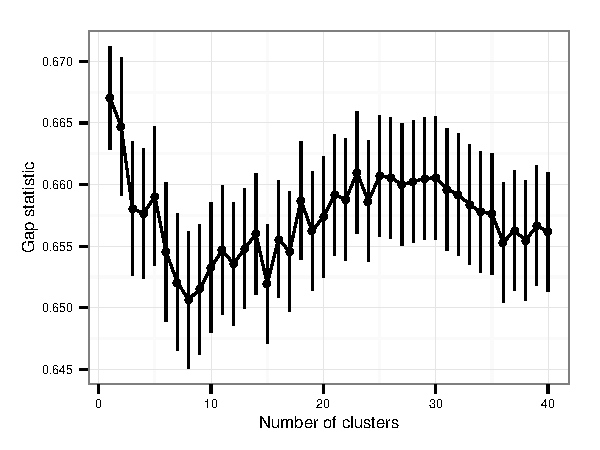
\includegraphics[width = \textwidth, keepaspectratio = true]{figure/gap}
  \caption{Gap statistic values for multiple PAM-based clustering configurations of the Riemmanian shape distances of the \textit{Emys marmorata} plastra. Higher values indicate greater clustering. Standard errors are estimated from 100 bootstrap resamples.}
  \label{fig:gap}
\end{figure}

Dissimilarity based EAC estimated approximately 5 optimal partitions (Table \ref{tab:dac}).

% latex table generated in R 2.15.3 by xtable 1.7-0 package
% Fri Apr  5 15:37:50 2013
\begin{table}[ht]
\begin{center}
\begin{tabular}{rr}
  \hline
 & tmorph.dac \\ 
  \hline
1 & 722 \\ 
  2 &   1 \\ 
  3 &   1 \\ 
  4 &   1 \\ 
  5 &   1 \\ 
   \hline
\end{tabular}
\caption{Number of specimens assigned to optimal number of partitions as determined by dissimilarity based EAC. Each column corresponds to a different partition, with the number assigned directly below it.}
\label{tab:dac}
\end{center}
\end{table}






\begin{figure}[ht]
  \centering
  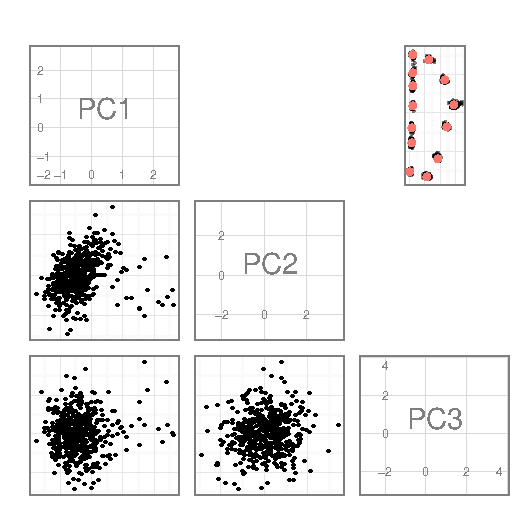
\includegraphics[width = \textwidth]{figure/gm}
  \caption{Visualization of PCA of \textit{E. marmorata}. The lower triangle is the pairwise comparison of the first three pricipal components. The upper left corner is the comparison of landmark dispersion for all specimens compared to the mean shape in red.}
  \label{fig:gm}
\end{figure}


\subsection{Supervised}

I'm currently holding back on showing the tables because there are a lot of them. I'll show the confusion matrix for the multinomial logicistic regressions because they are easy (Tables \ref{tab:multi-conf-sh1}, \ref{tab:multi-conf-sh2}, \ref{tab:multi-conf-sh3}, \ref{tab:multi-conf-spinks})

% latex table generated in R 2.15.3 by xtable 1.7-0 package
% Fri Apr  5 15:37:51 2013
\begin{table}[ht]
\begin{center}
\begin{tabular}{rrrr}
  \hline
 & CCR & marm & pall \\ 
  \hline
CCR &  40 &  14 &  11 \\ 
  marm &  25 &  74 &   2 \\ 
  pall &   3 &   1 &  10 \\ 
   \hline
\end{tabular}
\caption{Confusion matrix for sh1 classification scheme. Rows correspond to predicted class. Columns correspond to reference class.}
\label{tab:multi-conf-sh1}
\end{center}
\end{table}
% latex table generated in R 2.15.3 by xtable 1.7-0 package
% Fri Apr  5 15:37:51 2013
\begin{table}[ht]
\begin{center}
\begin{tabular}{rrrr}
  \hline
 & CCR & marm & pall \\ 
  \hline
CCR &  44 &  12 &  10 \\ 
  marm &  17 &  82 &   6 \\ 
  pall &   2 &   1 &   7 \\ 
   \hline
\end{tabular}
\caption{Confusion matrix for sh2 classification scheme. Rows correspond to predicted class. Columns correspond to reference class.}
\label{tab:multi-conf-sh2}
\end{center}
\end{table}
% latex table generated in R 2.15.3 by xtable 1.7-0 package
% Fri Apr  5 15:37:51 2013
\begin{table}[ht]
\begin{center}
\begin{tabular}{rrrrr}
  \hline
 & CCR & marm & pall & SJ \\ 
  \hline
CCR &  37 &  11 &   9 &   2 \\ 
  marm &  18 &  59 &   3 &  10 \\ 
  pall &   7 &   2 &  10 &   0 \\ 
  SJ &   1 &   4 &   1 &   7 \\ 
   \hline
\end{tabular}
\caption{Confusion matrix for sh3 classification scheme. Rows correspond to predicted class. Columns correspond to reference class.}
\label{tab:multi-conf-sh3}
\end{center}
\end{table}
% latex table generated in R 2.15.3 by xtable 1.7-0 package
% Fri Apr  5 15:37:51 2013
\begin{table}[ht]
\begin{center}
\begin{tabular}{rrrrr}
  \hline
 & 1 & 2 & 3 & 4 \\ 
  \hline
1 & 107 &   9 &  13 &  13 \\ 
  2 &   1 &   8 &   0 &   0 \\ 
  3 &   4 &   0 &   8 &   3 \\ 
  4 &   4 &   0 &   2 &   8 \\ 
   \hline
\end{tabular}
\caption{Confusion matrix for spinks classification scheme. Rows correspond to predicted class. Columns correspond to reference class.}
\label{tab:multi-conf-spinks}
\end{center}
\end{table}



But I can show the comparison of the predictive accuracies (Fig. \ref{fig:resamp}).




\begin{figure}[t]
  \centering
  \begin{subfigure}[b]{0.5\textwidth}
    \centering
    \caption{}
    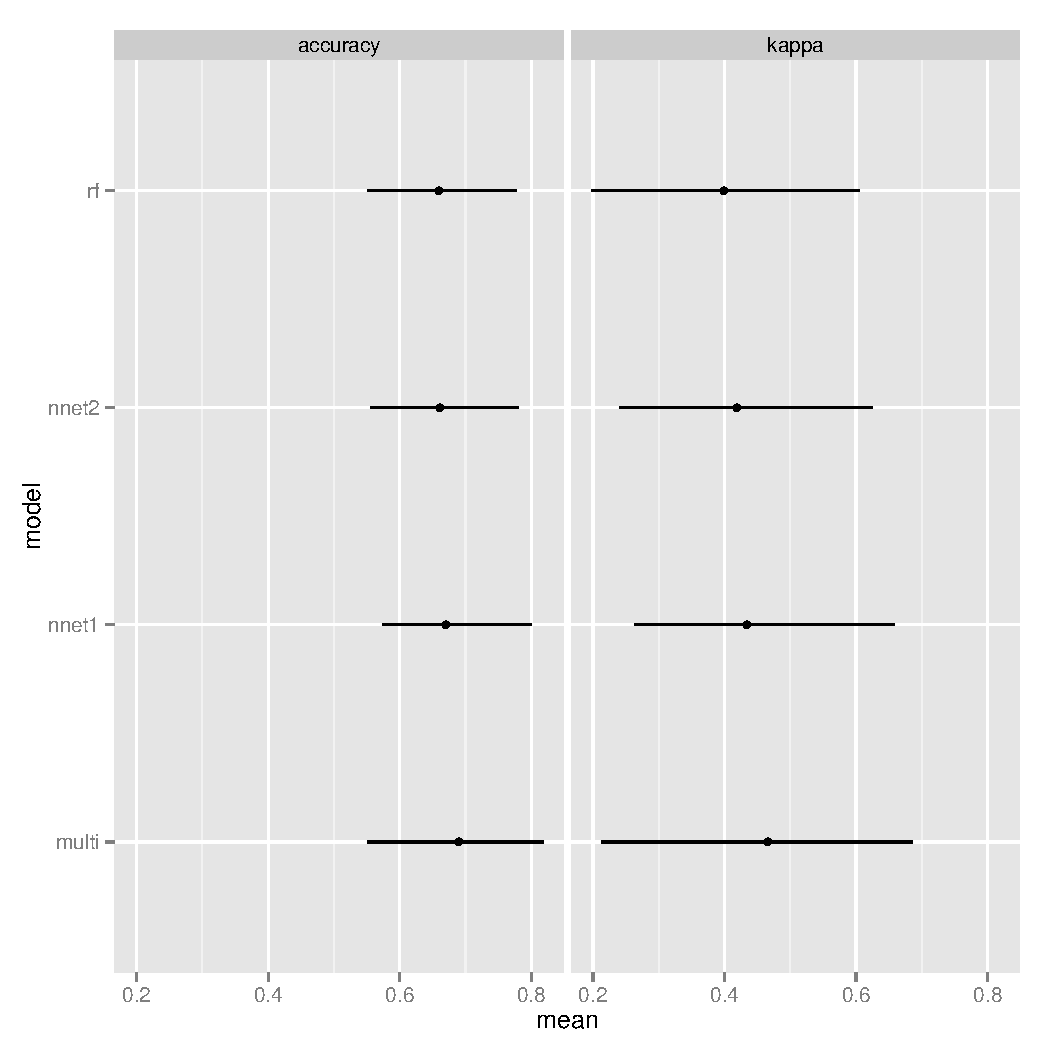
\includegraphics[width = \textwidth]{figure/resamp1}
    \label{fig:resamp1}
  \end{subfigure}%
  \begin{subfigure}[b]{0.5\textwidth}
    \centering
    \caption{}
    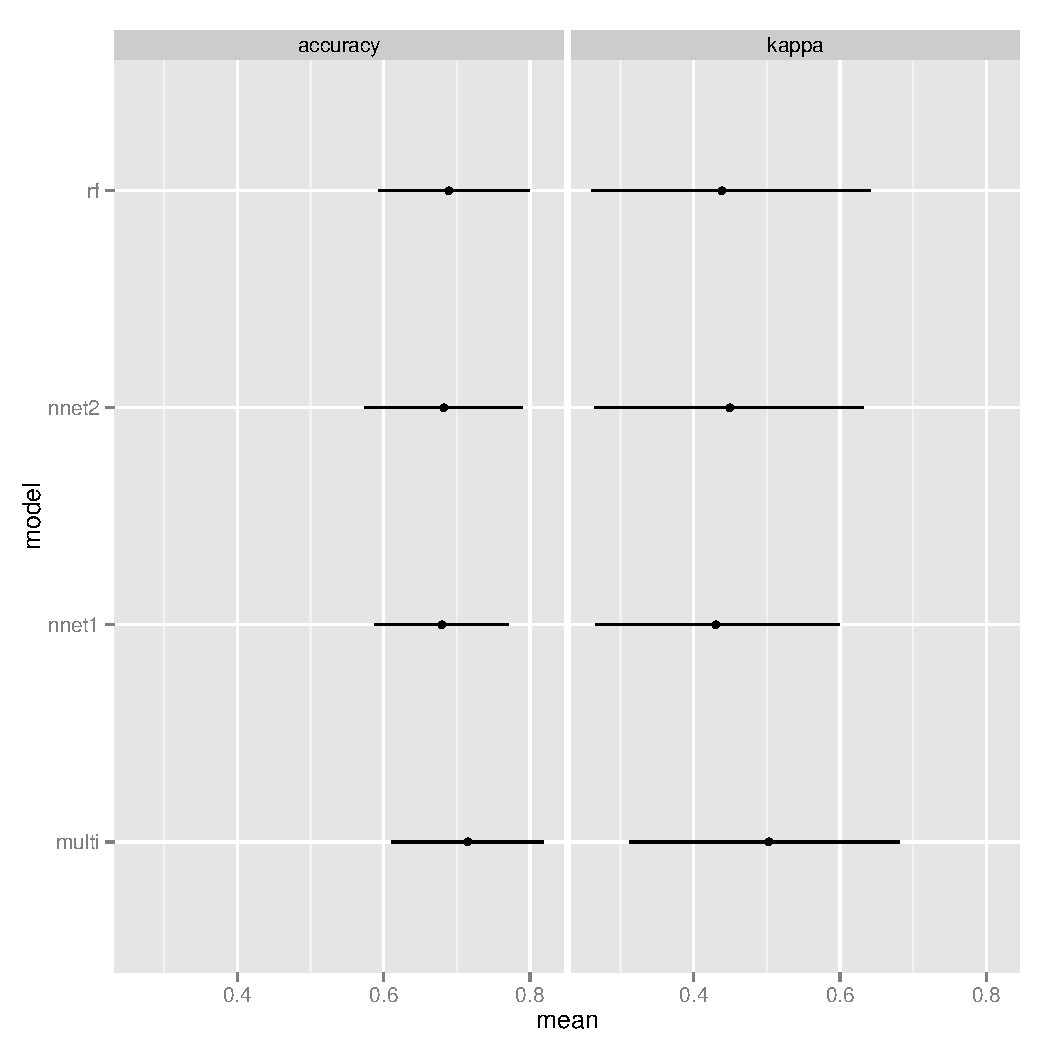
\includegraphics[width = \textwidth]{figure/resamp2}
    \label{fig:resamp2}
  \end{subfigure}\\

  \begin{subfigure}[b]{0.5\textwidth}
    \centering
    \caption{}
    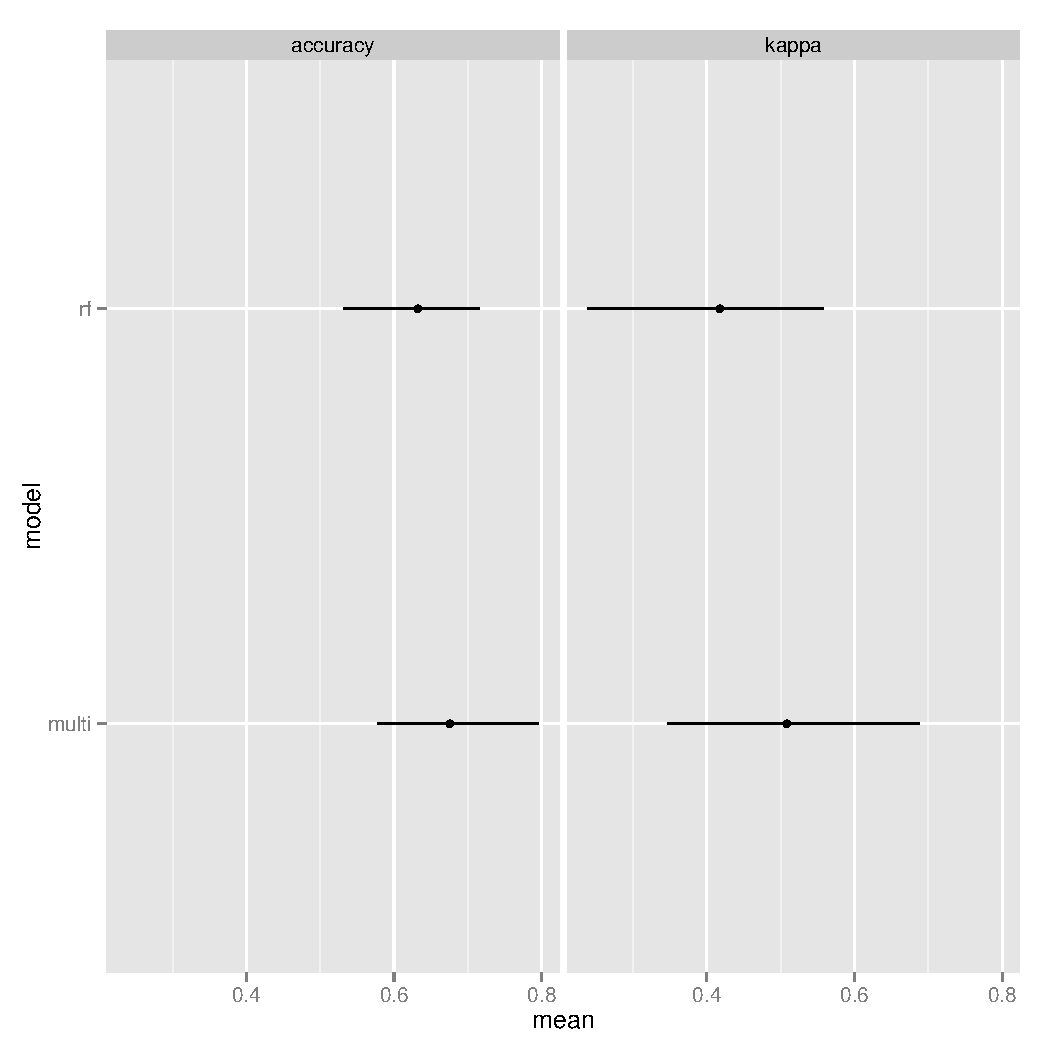
\includegraphics[width = \textwidth]{figure/resamp3}
    \label{fig:resamp3}
  \end{subfigure}%
  \begin{subfigure}[b]{0.5\textwidth}
    \centering
    \caption{}
    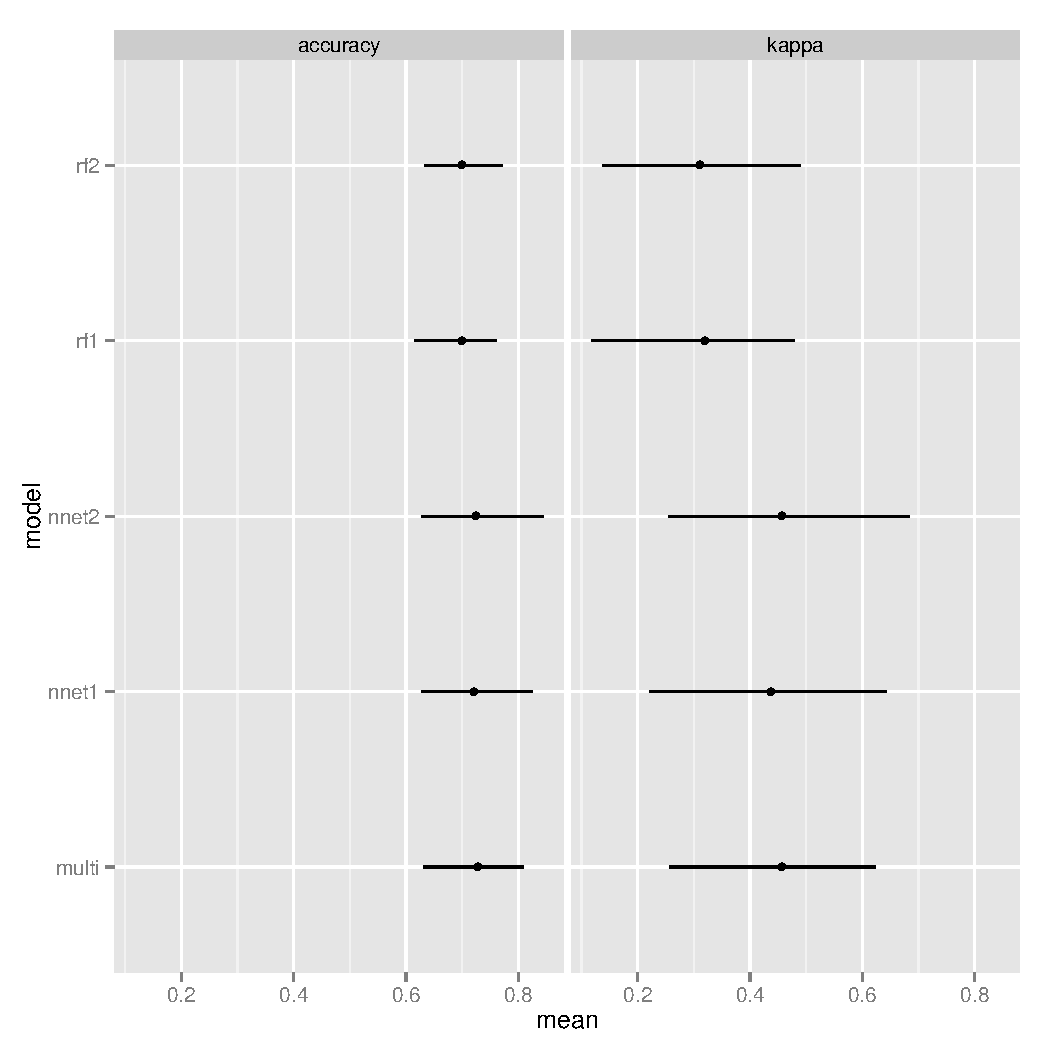
\includegraphics[width = \textwidth]{figure/resamp4}
    \label{fig:resamp4}
  \end{subfigure}
  \caption{Comparison of resampling distributions of training set accuracy and kappa statistics for the selected models of each classification scheme. \ref{fig:resamp1}: sh1 classification scheme. \ref{fig:resamp2}: sh2 classification scheme. \ref{fig:resamp3}: sh3 classification scheme. \ref{fig:resamp4}: spinks classification scheme.}
  \label{fig:resamp}
\end{figure}


In the interest of space/time, I'm only going to display results from one of the selected models from each method for each classification scheme.




\begin{figure}[t]
  \centering
  \begin{subfigure}[b]{0.5\textwidth}
    \centering
    \caption{}
    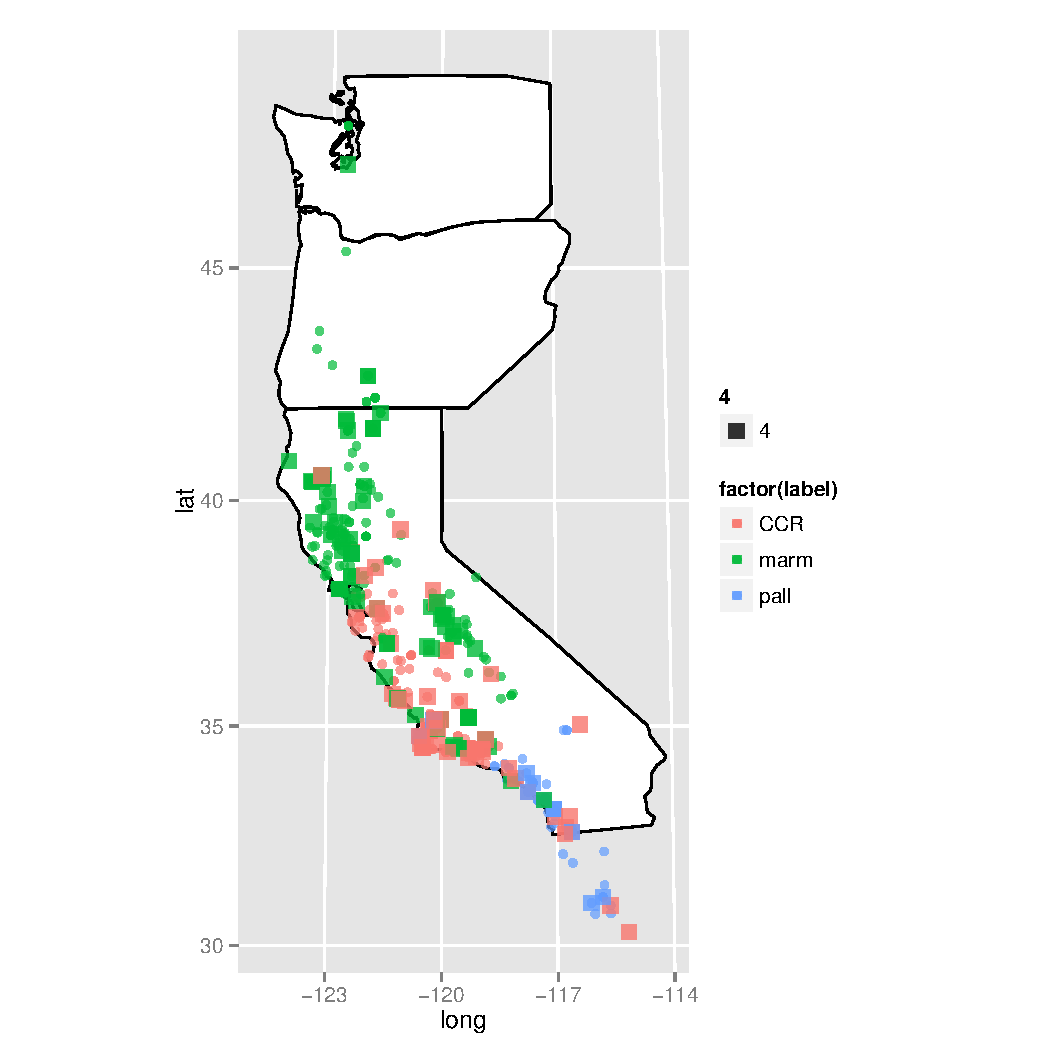
\includegraphics[width = \textwidth]{figure/multi-map1}
    \label{fig:multi-map1}
  \end{subfigure}%
  \begin{subfigure}[b]{0.5\textwidth}
    \centering
    \caption{}
    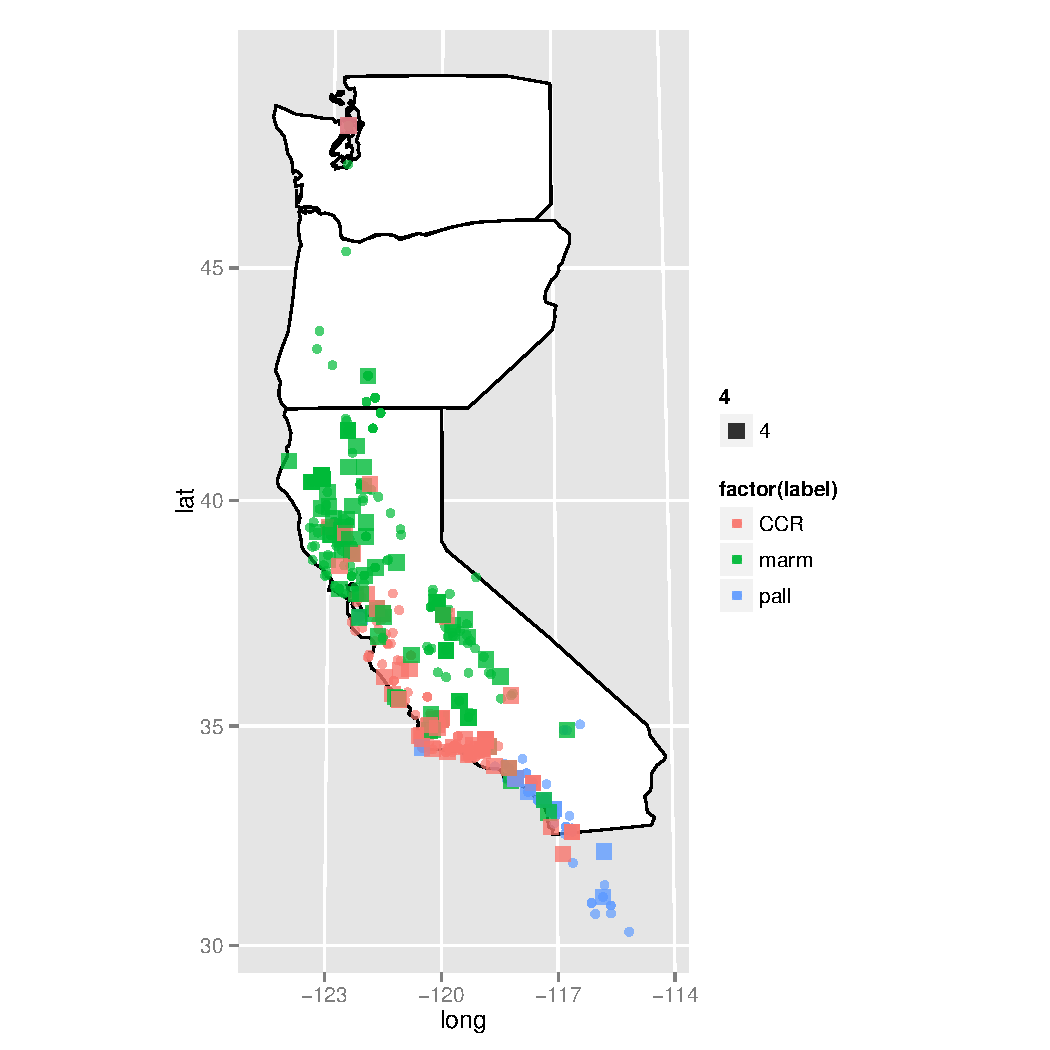
\includegraphics[width = \textwidth]{figure/multi-map2}
    \label{fig:multi-map2}
  \end{subfigure}\\

  \begin{subfigure}[b]{0.5\textwidth}
    \centering
    \caption{}
    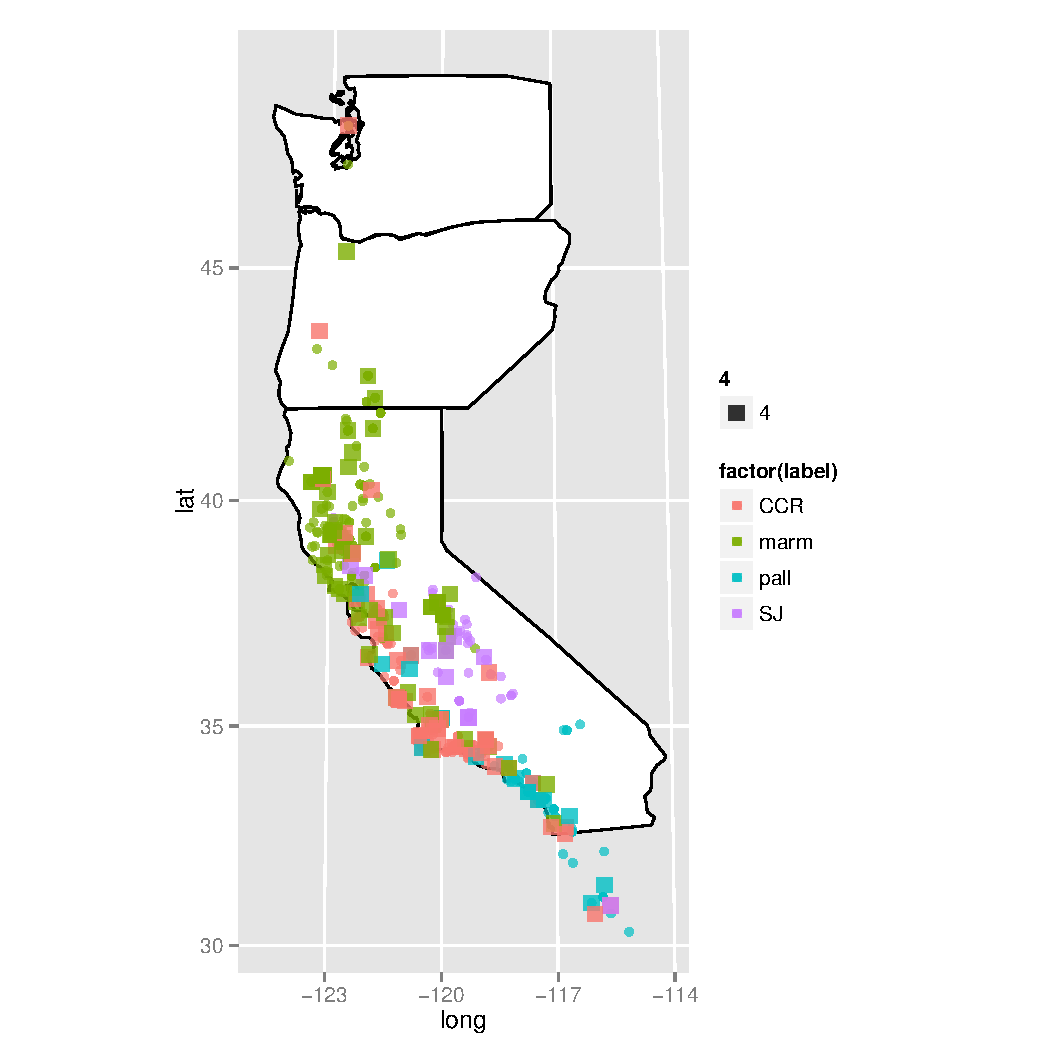
\includegraphics[width = \textwidth]{figure/multi-map3}
    \label{fig:multi-map3}
  \end{subfigure}%
  \begin{subfigure}[b]{0.5\textwidth}
    \centering
    \caption{}
    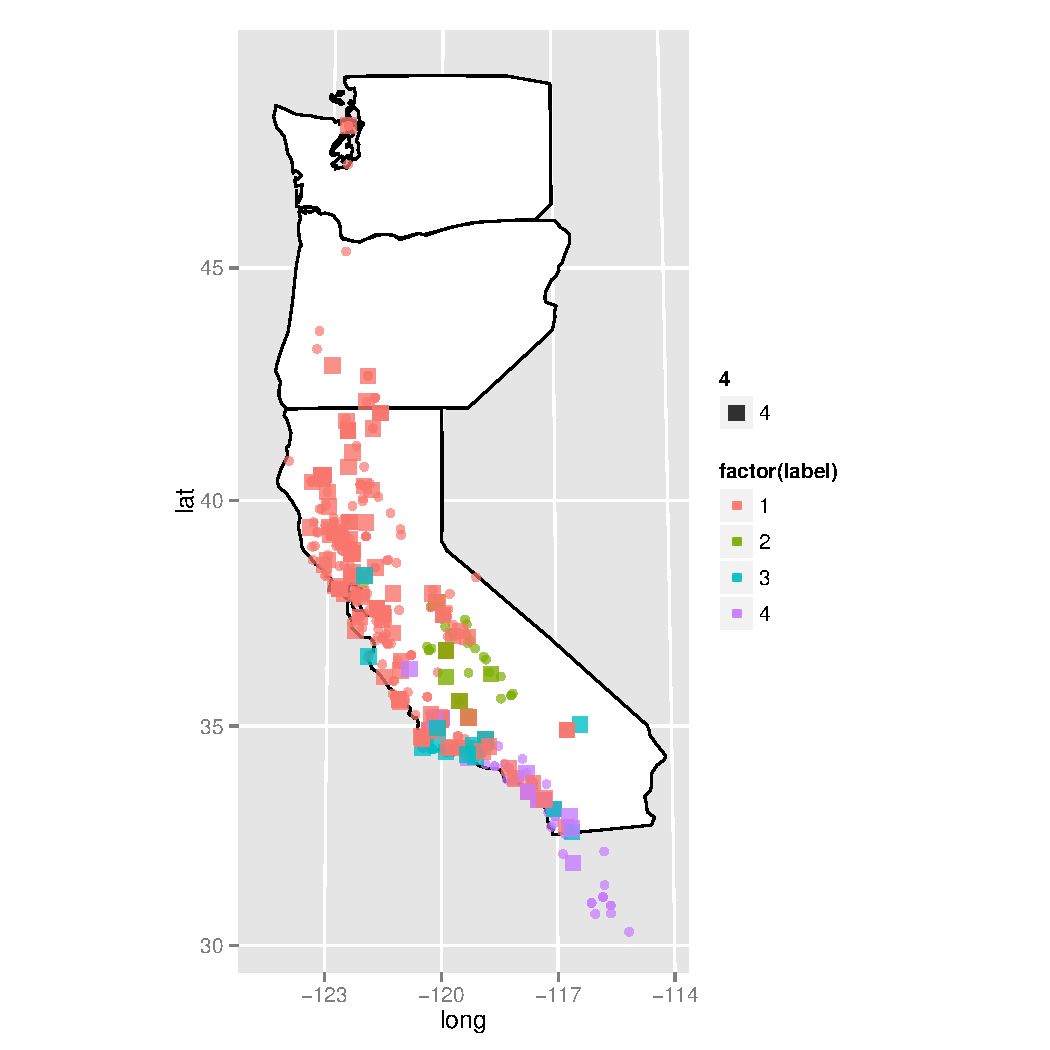
\includegraphics[width = \textwidth]{figure/multi-map4}
    \label{fig:multi-map4}
  \end{subfigure}
  \caption{Geographic position of all turtles sampled. Both training and testing observations are plotted. Training set observations are circles while testing observations are larger squares. Testing set observations are classified based on a multinomial logistic regression model. \ref{fig:multi-map1}: sh1 classification scheme. \ref{fig:multi-map2}: sh2 classification scheme. \ref{fig:multi-map3}: sh3 classification scheme. \ref{fig:multi-map4}: spinks classification scheme.}
  \label{fig:multi-map}
\end{figure}




\begin{figure}[t]
  \centering
  \begin{subfigure}[b]{0.5\textwidth}
    \centering
    \caption{}
    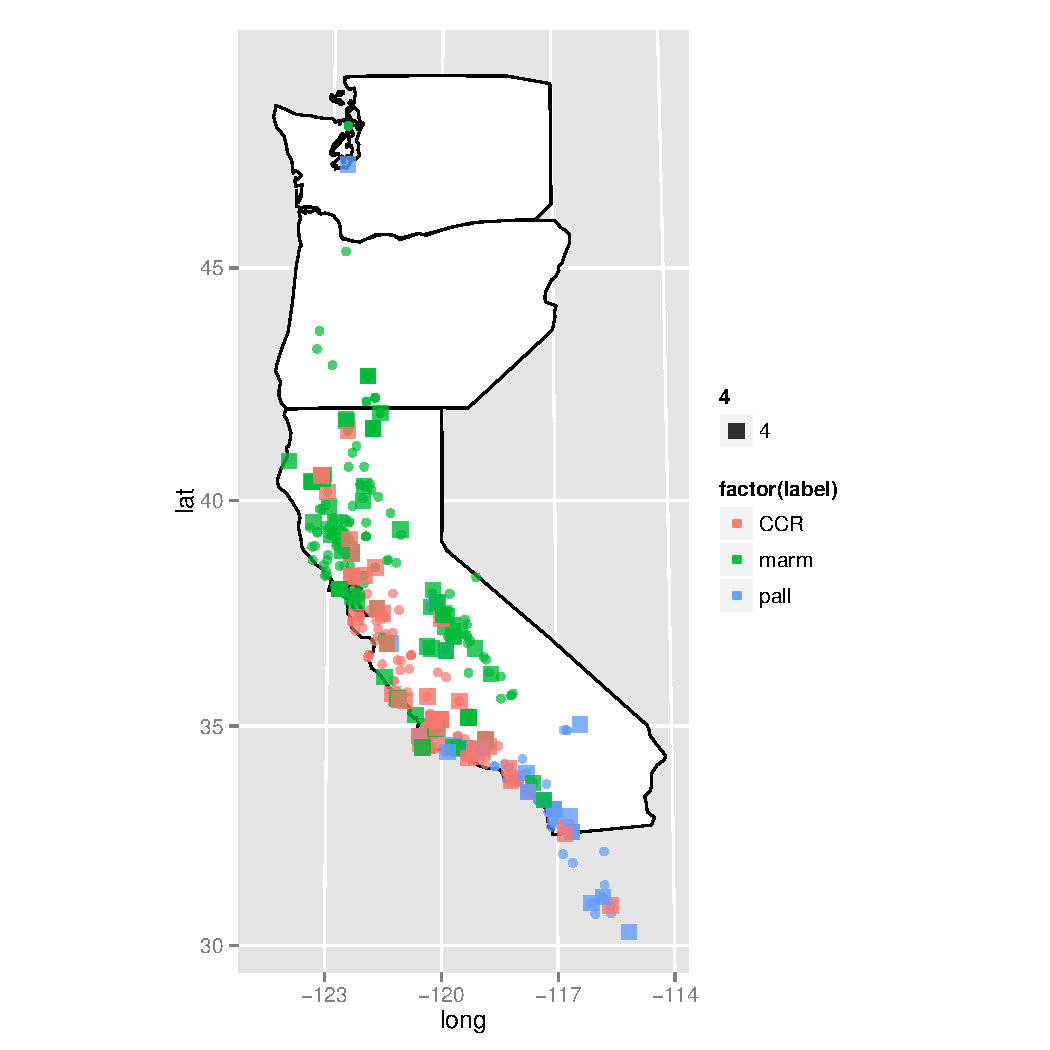
\includegraphics[width = \textwidth]{figure/nnet-map1}
    \label{fig:nnet-map1}
  \end{subfigure}%
  \begin{subfigure}[b]{0.5\textwidth}
    \centering
    \caption{}
    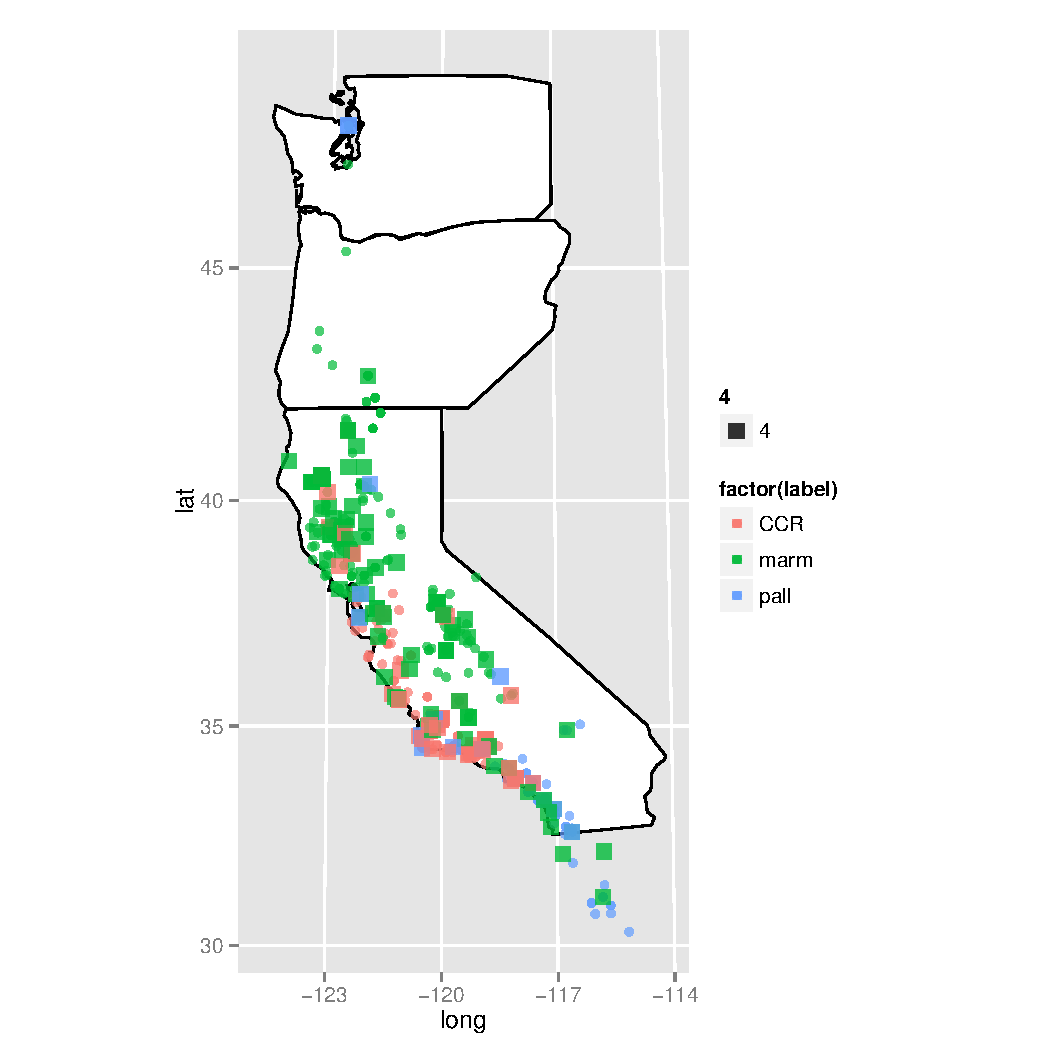
\includegraphics[width = \textwidth]{figure/nnet-map2}
    \label{fig:nnet-map2}
  \end{subfigure}\\

  \begin{subfigure}[b]{0.5\textwidth}
    \centering
    \caption{}
    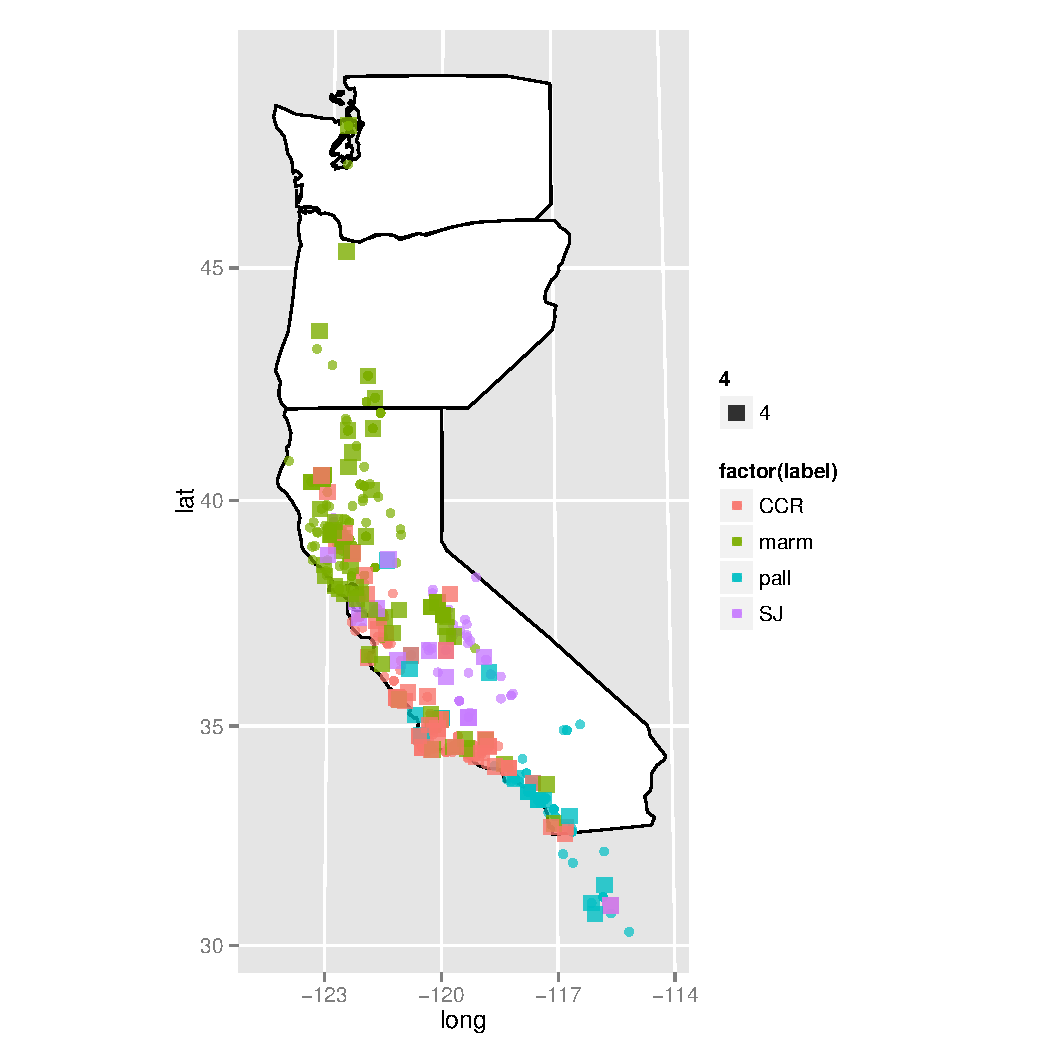
\includegraphics[width = \textwidth]{figure/nnet-map3}
    \label{fig:nnet-map3}
  \end{subfigure}%
  \begin{subfigure}[b]{0.5\textwidth}
    \centering
    \caption{}
    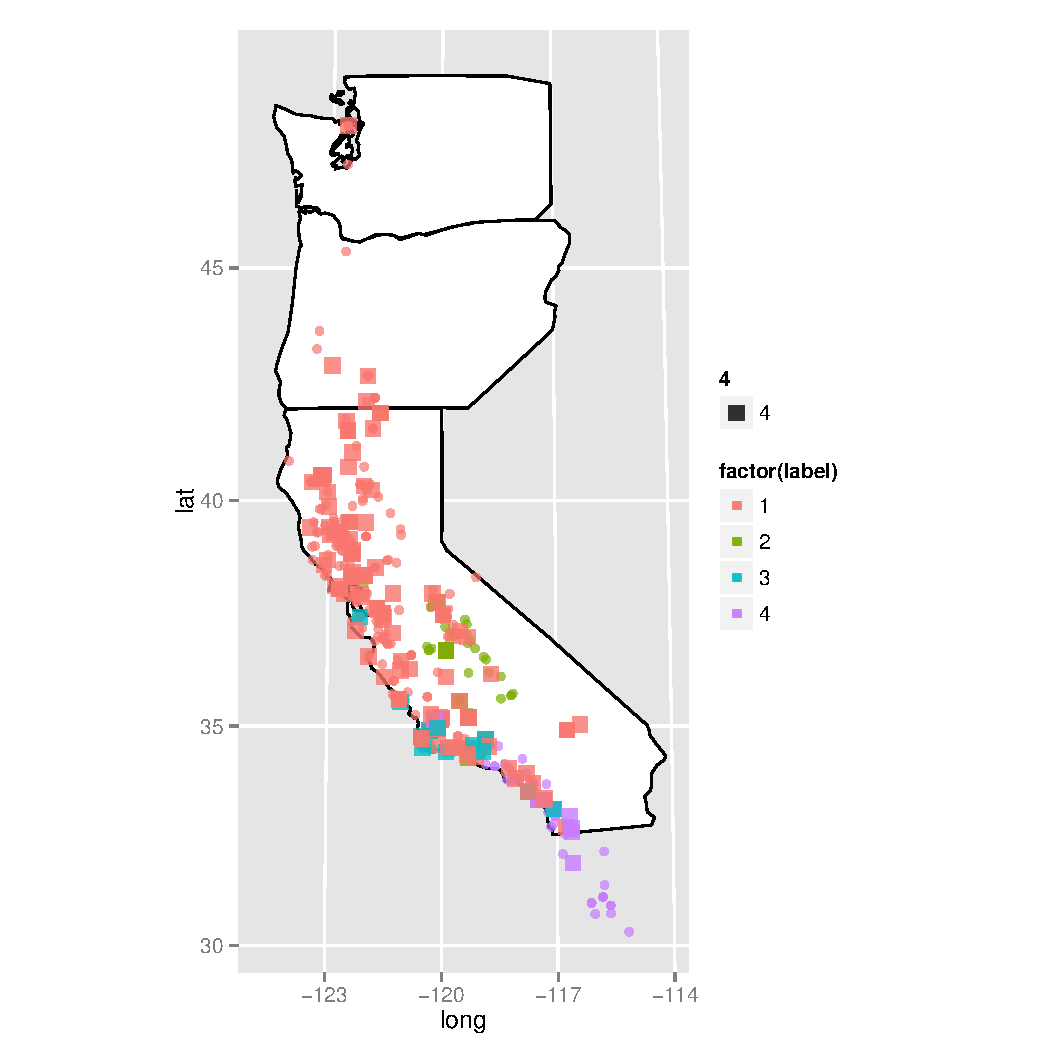
\includegraphics[width = \textwidth]{figure/nnet-map4}
    \label{fig:nnet-map4}
  \end{subfigure}
  \caption{Geographic position of all turtles sampled. Both training and testing observations are plotted. Training set observations are circles while testing observations are larger squares. Testing set observations are classified based on a feed-forward single layer neural network model. \ref{fig:nnet-map1}: sh1 classification scheme. \ref{fig:nnet-map2}: sh2 classification scheme. \ref{fig:nnet-map3}: sh3 classification scheme. \ref{fig:nnet-map4}: spinks classification scheme.}
  \label{fig:nnet-map}
\end{figure}





\begin{figure}[t]
  \centering
  \begin{subfigure}[b]{0.5\textwidth}
    \centering
    \caption{}
    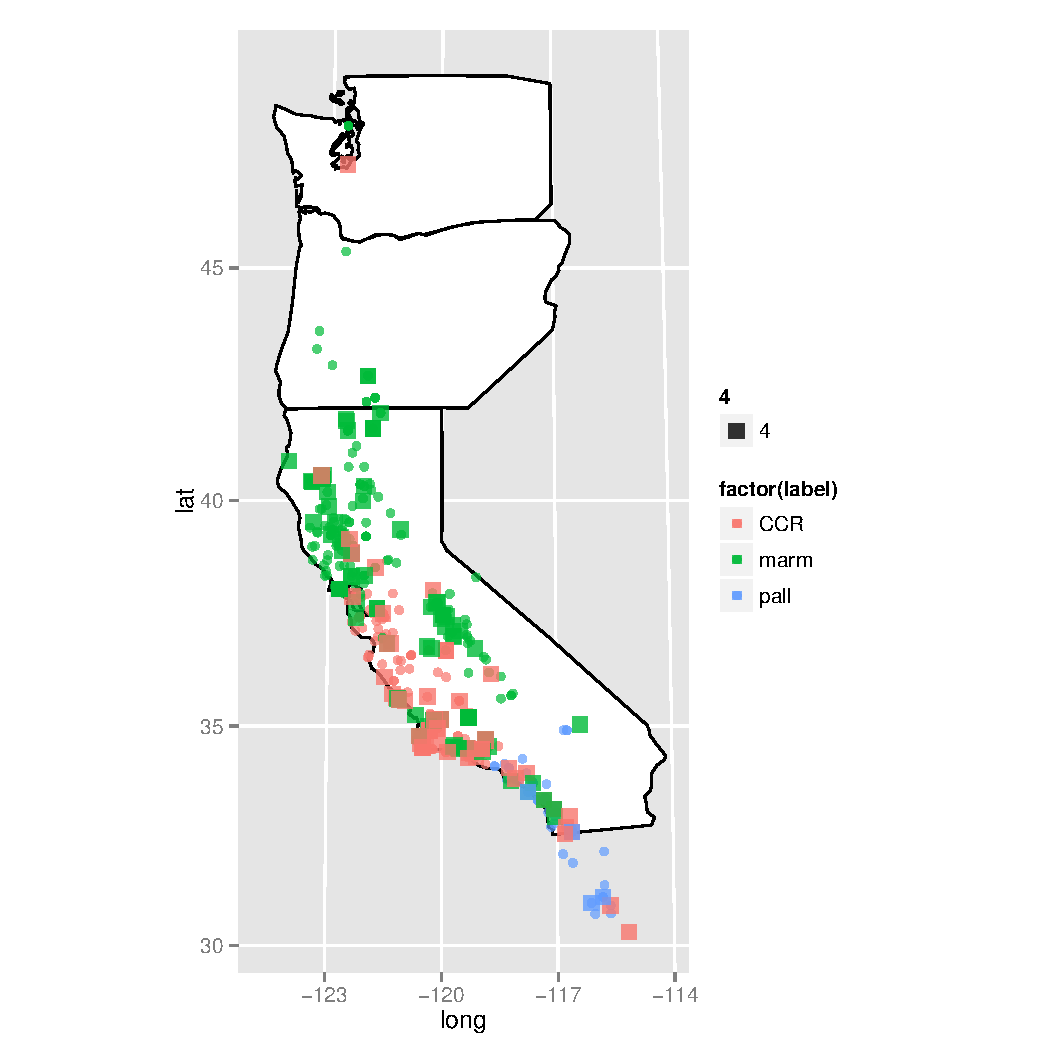
\includegraphics[width = \textwidth]{figure/rf-map1}
    \label{fig:rf-map1}
  \end{subfigure}%
  \begin{subfigure}[b]{0.5\textwidth}
    \centering
    \caption{}
    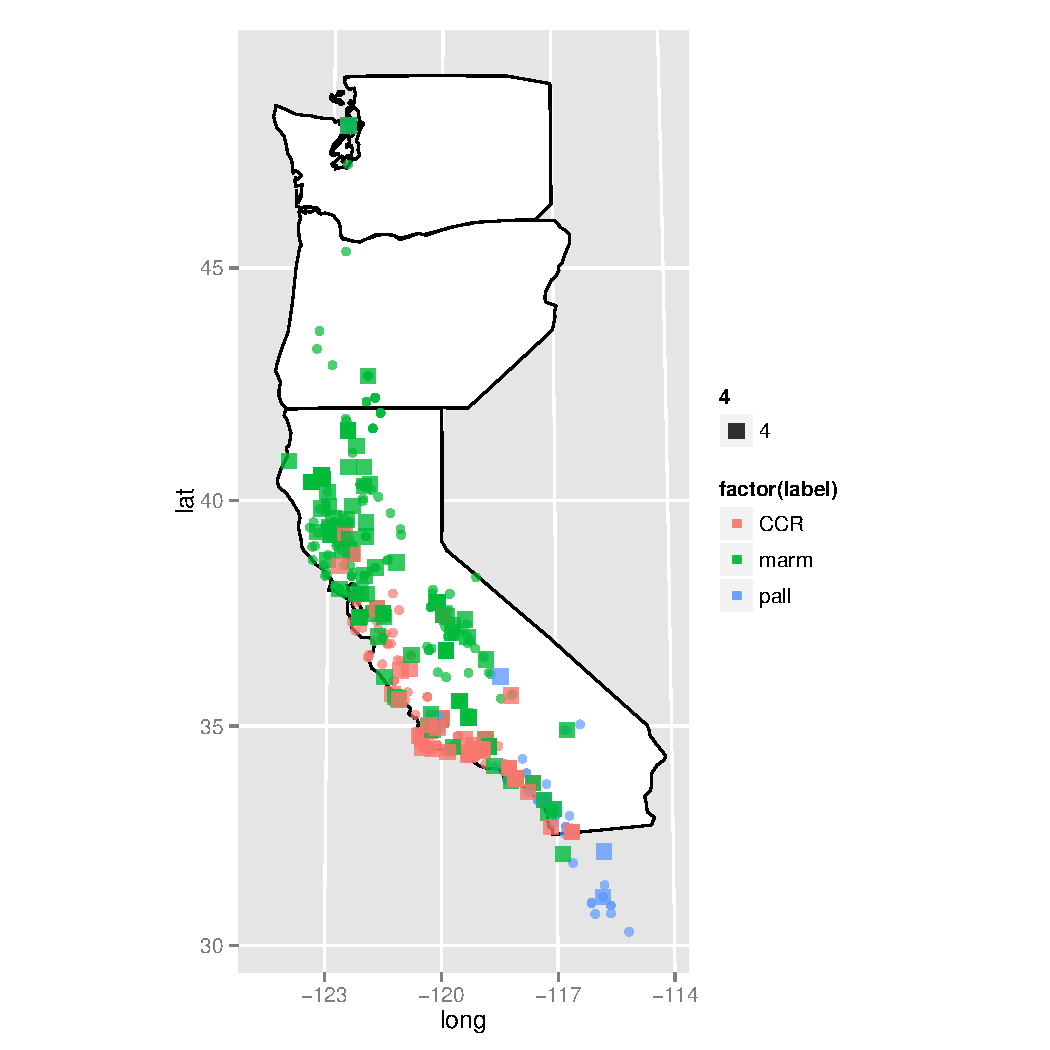
\includegraphics[width = \textwidth]{figure/rf-map2}
    \label{fig:rf-map2}
  \end{subfigure}\\

  \begin{subfigure}[b]{0.5\textwidth}
    \centering
    \caption{}
    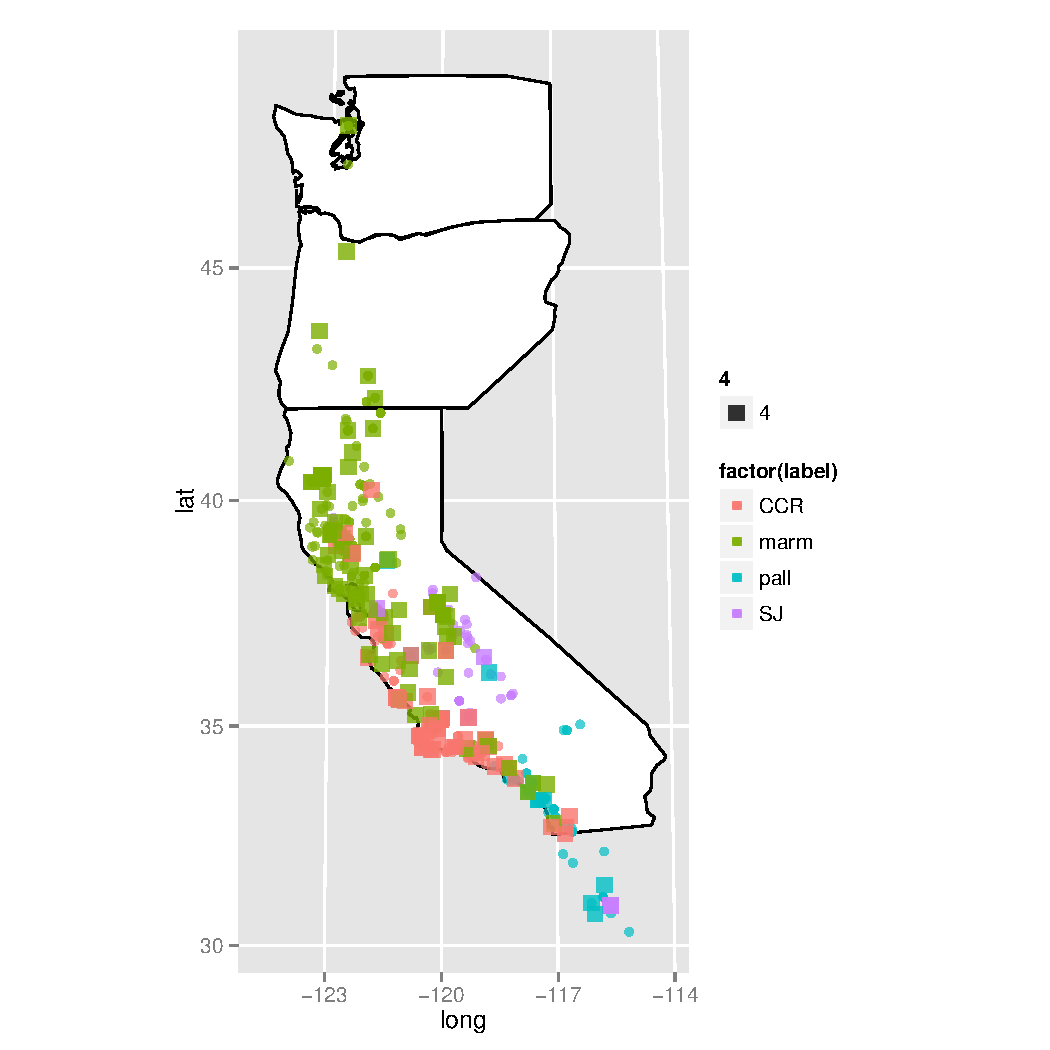
\includegraphics[width = \textwidth]{figure/rf-map3}
    \label{fig:rf-map3}
  \end{subfigure}%
  \begin{subfigure}[b]{0.5\textwidth}
    \centering
    \caption{}
    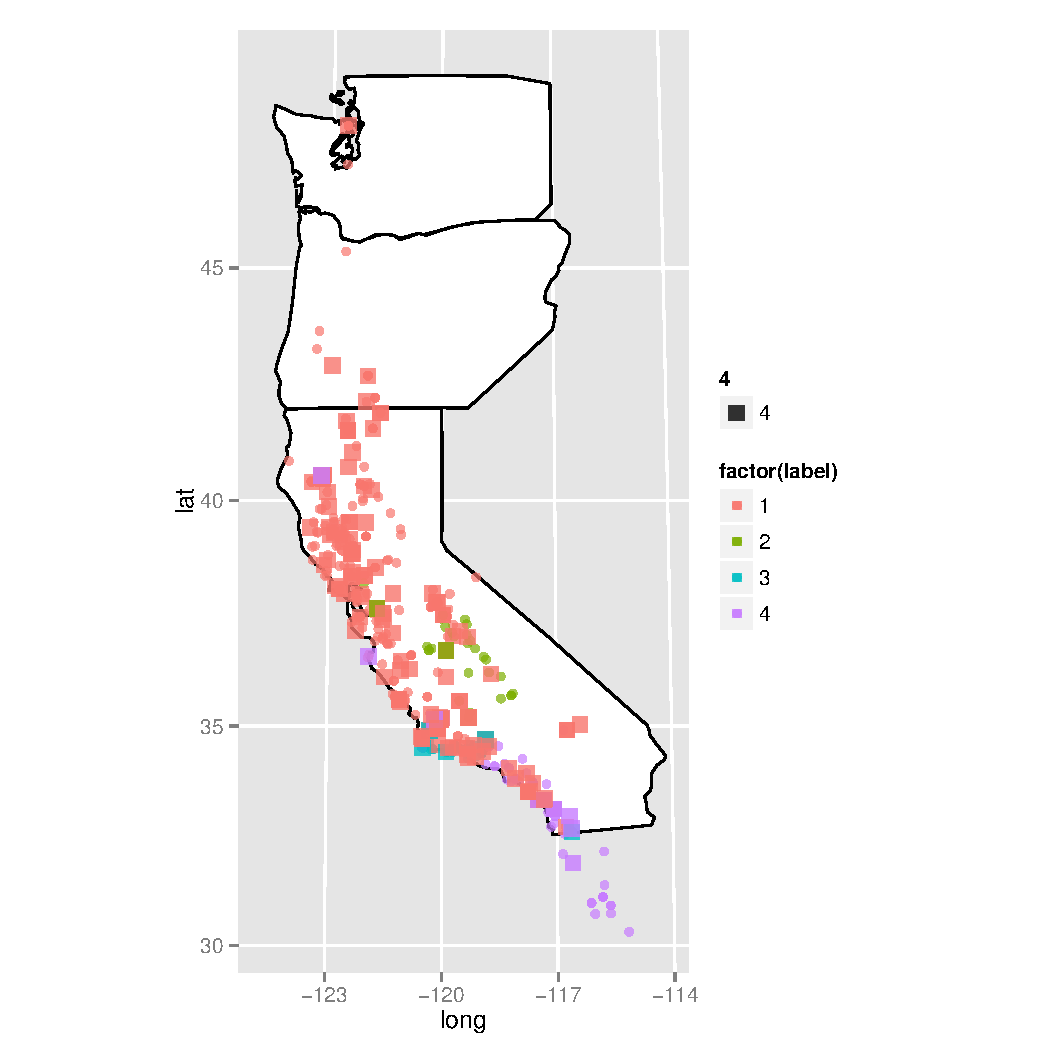
\includegraphics[width = \textwidth]{figure/rf-map4}
    \label{fig:rf-map4}
  \end{subfigure}
  \caption{Geographic position of all turtles sampled. Both training and testing observations are plotted. Training set observations are circles while testing observations are larger squares. Testing set observations are classified based on a random forest model. \ref{fig:rf-map1}: sh1 classification scheme. \ref{fig:rf-map2}: sh2 classification scheme. \ref{fig:rf-map3}: sh3 classification scheme. \ref{fig:rf-map4}: spinks classification scheme.}
  \label{fig:rf-map}
\end{figure}


\section{Future}
\begin{enumerate}
  \item remove juvelines
  \item look into multinomial logistic mixed-effects models
  \item other unsupervised methods, though that might have to wait for a follow up paper
    \begin{itemize}
      \item bayesian nonparametrics for categorical data
    \end{itemize}
\end{enumerate}

In general, misclassification seems to be at random. This is interesting for a few reasons. The assignments based on geography do not seem to bias results. All the taxa are extremely similar, though there are differences, hence the ~70\% accuracy. None of the classification schemes seems necessary better than any of the others, though sh3 is probably the best (4 classes) over all because it is the least ``random''. I think there is a summary class specific statistic that better explains this (sensitivity? specificity? detection rate?). These will illuminate which classes are ``strongest''.

\section{Miscellaneous affairs}
\subsection{Evolution 2013}
How cryptic is cryptic diversity? Machine learning approaches to fine scale variation in the morphology of \textit{Emys marmorata}.


\subsection{Grants}
\subsubsection{Hinds Fund}
Resubmit previous application with the results from this study in the prelim-results section?

Get network for one turtle? This should take long, just requires time.

Other project ideas I've come up with over the last few months that might be alternatives to the turtle shell network project.

\begin{itemize}
  \item NA terrestrial mammal community change in the Eocene. Using clustering/unsupervised methods, classify the sites in the Eocene. Spatio-temporal dynamics? Using co-occurrence networks and bipartite site-networks to understand spatio-temporal dynamics in paleo-community structure.
  \item South African P/T faunal zones. Do my methods to the faunal assemblages. Sidor in press makes conclusions about how hard it is to identify some zones as opposed to others because of mixing. Do predictive methods agree? This is another nice spatio-temporal dynamics project.
  \item Character correlation and nonindependence. I did half my masters on this stuff. Using frequent pattern mining algorithms and nonparametric Bayesian approaches it may be possible to revisit these ideas with actual results.
  \item Revisit Wagner 2000 idea of character and character state exhaustion. Expand into the realm of uncertainty using stochastic character mapping. Potential also with chinese restaurant/indian buffet processes as models of character addition though this is highly suspect.
\end{itemize}

The three of these have at least preliminary methods/results, so they might be more appealing for the Hinds Fund. The concern becomes what do I actually need money for? Currently, my ideas are monitor, keyboard, mouse, hard drive, wrist bands (I have wrist pain). Publication and conference costs aren't appropriate for the Hinds, which is very frustrating because that's where most of my money goes.

I still can't believe I was rejected last round.

\subsubsection{Paleontological Society}
Why not? Need to wait till next year. Should probably join PaleoSoc anyway.


\end{document}
